\chapter{Models}
Let's begin the chapter with a question. Why do we need models?
Well, they represent a good approximation of the real world and allow describing events through a parametric representation (parameters can be extracted and used for processing). In the context of computer vision, models are used to describe the geometry of the world, the appearance of objects, and the imaging process. In this chapter, we will discuss the most common models used in computer vision. We will start with the pinhole camera model, then we will see the perspective projection model and finally, we will discuss the appearance model.
\section{The Pinhole Camera Model}
The pinhole camera model is the simplest model used to describe the imaging process. It is based on the principle that light travels in straight lines. The model is composed of a pinhole, a plane, and an image plane. The pinhole is a small hole in the plane, and the image plane is placed behind the pinhole. The light rays coming from the scene pass through the pinhole and project the scene onto the image plane. 
\\\textit{PS: If the object is far, it appears small in the image. If the object is close, it appears large in the image.}
\subsection{Features of the Pinhole Camera Model}
In an image, parallel lines in the real world converge at a single point, known as the vanishing point. Parallel lines on the same plane converge to collinear vanishing points, forming a line called the horizon for that plane. Additionally, vertical lines in the image are perpendicular to this horizon. 

\subsection{Features of the Pinhole Camera Model}

\begin{figure}[H]
    \centering
    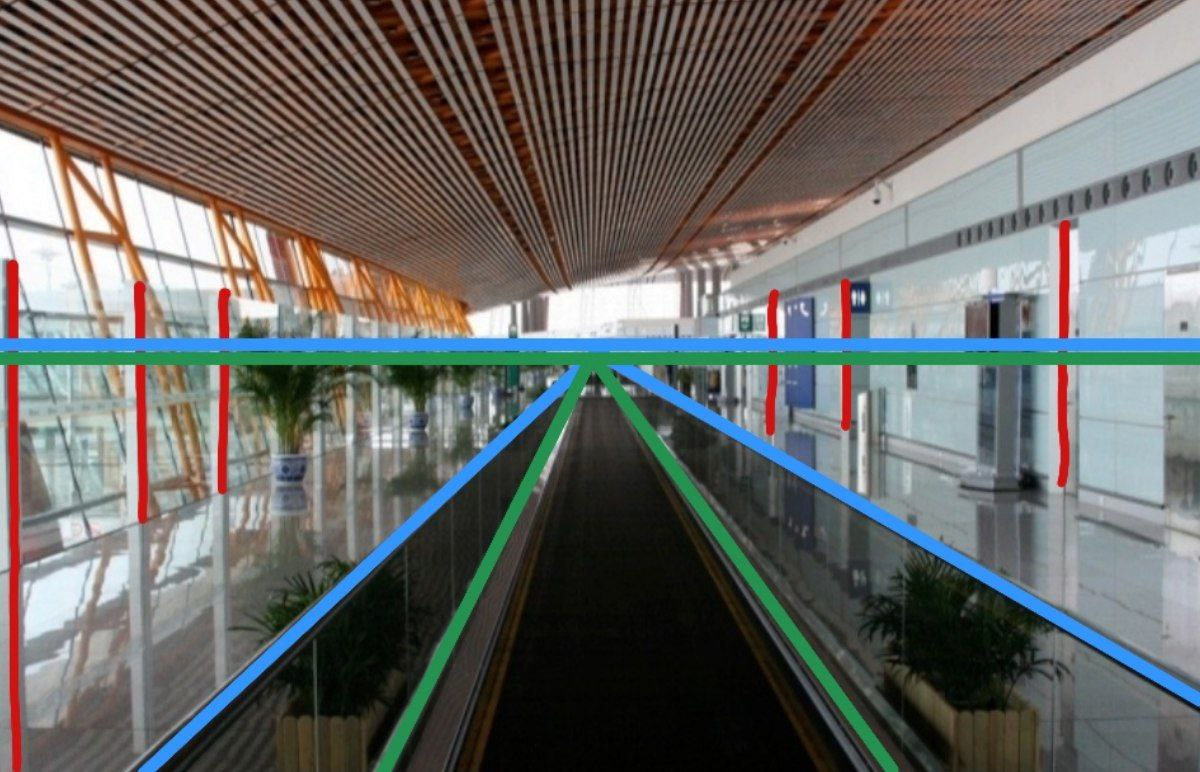
\includegraphics[width=0.5\textwidth]{Figures/horizon.jpg}
    \caption{The behavior of parallel lines in the world and in the image.}
    \label{fig:horizon}
\end{figure}
\begin{itemize}
    \item Parallel lines in the world converge to a single point in the image;
    \item Parallel lines on the same plane lead to \textit{collinear vanishing} points. In Figure \ref{fig:horizon} we can see how the blue and green lines, that lie parallel on two different planes, eventually converge to the same point in the image plane;
    \item The line where coplanar parallel lines end up is called the \textit{horizon} for that plane;
    \item Vertical lines (red) are perpendicular to the horizon.
\end{itemize}

\begin{figure}[H]
    \centering
    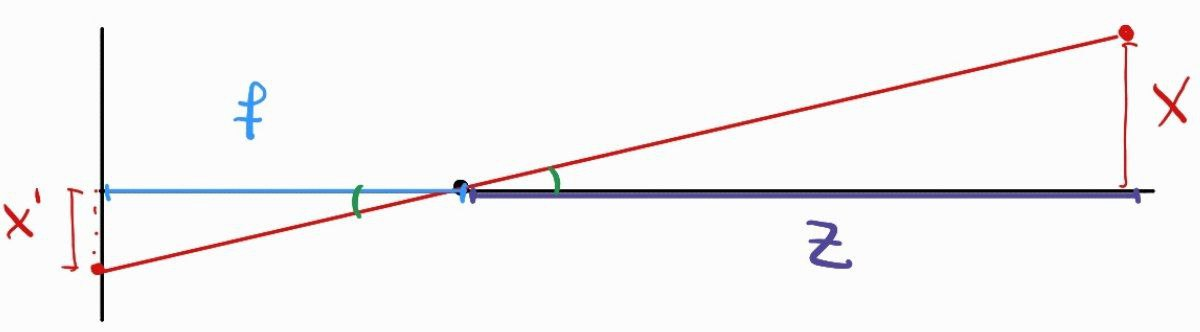
\includegraphics[width=0.5\textwidth]{Figures/triangles.jpg}
    \caption{Similar triangles in the projection.}
    \label{fig:triangles}
\end{figure}

The intuition behind the projection of the pinhole camera model is based on the concept of similar triangles. In Figure \ref{fig:triangles} we can see how the triangles formed by the object and the image plane are similar, \(f\) is the \textit{focal length} of the camera, \(Z\) is the distance of the object to the pinhole and \(X\) and \(X'\) are respectively the position of the object and its projection on the image plane. This means that the ratio of the sides of the triangles is the same, this concept is used to derive the projection equations. 

\begin{figure}[H]
    \centering
    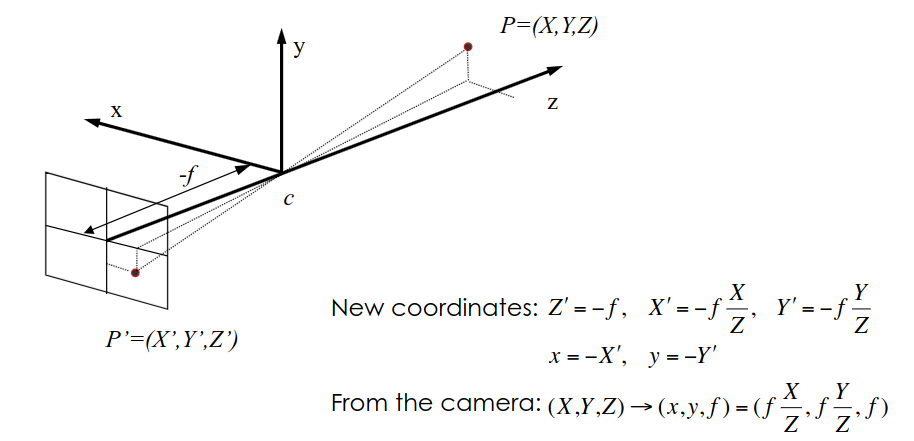
\includegraphics[width=1\textwidth]{Figures/Pinhole.png}
    \caption{If the object is far, it appears small in the image. If the object is close, it appears large in the image.}
\end{figure}
\section{Projection}
Projection is the fundamental process of mapping 3D points, including time, to 2D points. When projecting a 3D point onto the image plane, a line is defined between the point and the center of projection. The intersection of this line with the image plane yields the 2D projection of the 3D point. This process forms the basis of how 3D scenes are represented in 2D images.
\[
    f: \mathbb{R}^4 \rightarrow \mathbb{R}^3    
\]
\[
    f(X,Y,Z,t) = (x,y,t)
\]
\textit{NB: These are continuous variables.}       
\\
There exist two types of projection:
\begin{itemize}
    \item Perspective projection;
    \item Orthographic projection.
\end{itemize}
\subsection{The Perspective Projection Model}
The perspective projection model is an extension of the pinhole camera model. It is used to describe the imaging process in a more realistic way. The model is based on the principle that light travels in straight lines and that the image is formed by the intersection of these lines with the image plane. 
For simplicity, we usually consider the image plane on the same side of the “real world”, to avoid the picture flip.\\\\
\begin{figure}[H]
    \begin{subfigure}{0.5\textwidth}
        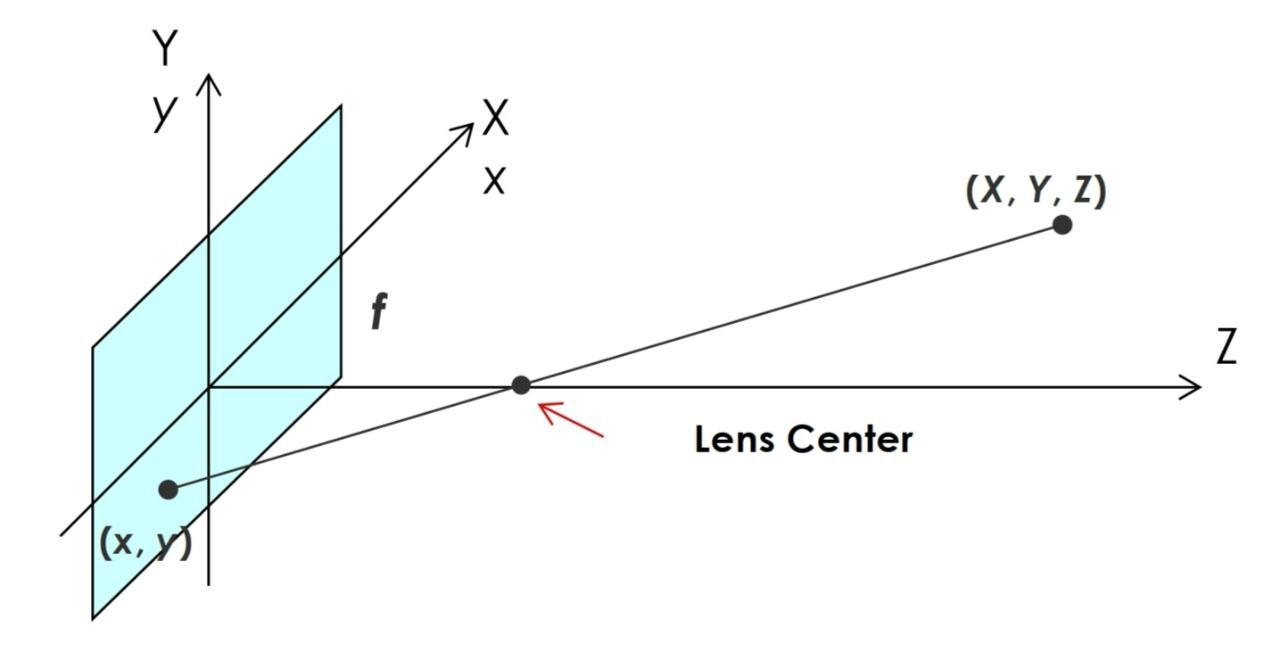
\includegraphics[scale=0.2]{Figures/Perspective_proj1.jpeg}
        \caption{The pinhole camera model.} 
        \label{fig:subim1}
    \end{subfigure}
    \begin{subfigure}{0.5\textwidth}
        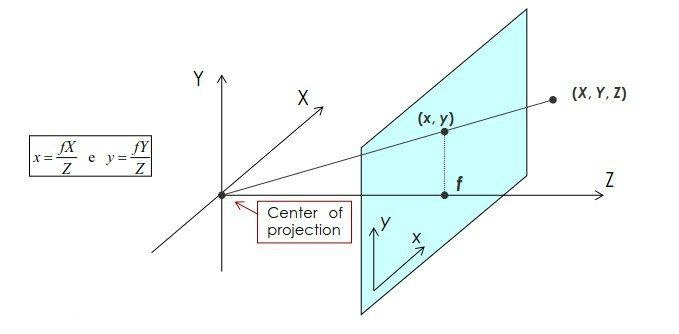
\includegraphics[scale=0.4]{Figures/Perspective_proj.jpeg}
        \caption{The perspective projection model.}
        \label{fig:subim2}
    \end{subfigure}
    \caption{We can see how in \ref{fig:subim2} we moved the camera plane on the right side and the center of projection at the origin, for this reason a $-f$ is added to the denominator.}
        \label{fig:image2}
\end{figure}


\[
    \begin{cases}
        \frac{x}{f} = \frac{X}{Z-f} \\
        \frac{y}{f} = \frac{Y}{Z-f}
    \end{cases} \Rightarrow \begin{cases}
        x = \frac{fX}{Z-f} \\
        y = \frac{fY}{Z-f}
    \end{cases} \Rightarrow \begin{cases}
        x = \frac{fX}{Z} \\
        y = \frac{fY}{Z}
    \end{cases}
\]

Now the center of projection corresponds to the origin of the 3D space, and the plane $(X,Y)$ is parallel to $(x,y)$. From a computational point of view nothing changes, we simply shift the image plane from back to front in order to have the image straight. Due to the fact that we assume that $f$ is negletable, compared to Z (Z$>>$f) we can safely approximate the denominator and remove the $-f$, obtaining the same equations as the pinhole camera model.


\subsection{The Orthographic Projection Model}
The orthographic projection model is a simplified version of the perspective projection model. It is assumed that all rays originated from the 3D object, and from the scene in general, are parallel among each other. 
In the drawing, the image plane is parallel to $(X,Y)$.
\begin{figure}[h]
    \centering
    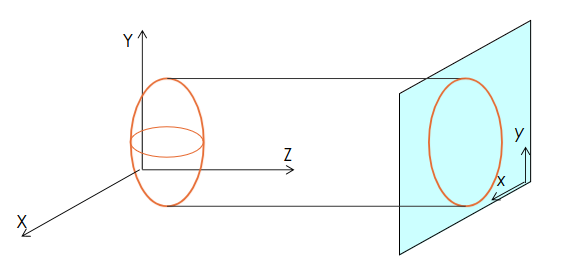
\includegraphics[width=0.5\textwidth]{Figures/Orthographic_proj.png}
\end{figure}
\\Assuming this, the orthographic projection
can be simply described in Cartesian coordinates as:
\[
    \begin{cases}
        x = X \\
        y = Y
    \end{cases}
\]
Or in form of a matrix:
\[
    \begin{bmatrix}
        x \\
        y
    \end{bmatrix} = \begin{bmatrix}
        1 & 0 & 0 \\
        0 & 1 & 0
    \end{bmatrix} \begin{bmatrix}
        X \\
        Y \\
        Z
    \end{bmatrix}   
\]
\textit{NB: The distance of the object from the camera does not affect the intensity of the image projected onto the 2D plane.
It is a good approximation when the distance of the object is much bigger than the depth of the object itself. }

\section{Illumination Models}
Illumination plays a crucial role in how we perceive objects, as it defines their appearance. 
When a light source interacts with an object, light can be absorbed, reflected, or transmitted. 
Modeling illumination is complex because we perceive objects based on how they reflect light across specific wavelengths. 
Remember that reflection can be either specular or diffuse.

Specular reflection concentrates more energy in the direction of the light source, creating highlights. 
Conversely, diffuse reflection distributes energy uniformly in all directions, making the position of the observer irrelevant. 

Surfaces vary in specularity: matte surfaces reflect light uniformly, while glossy ones reflect light directionally. 
The specularity also depends on factors such as surface distance and the angle of the light source.

\begin{figure}[H]
    \centering
    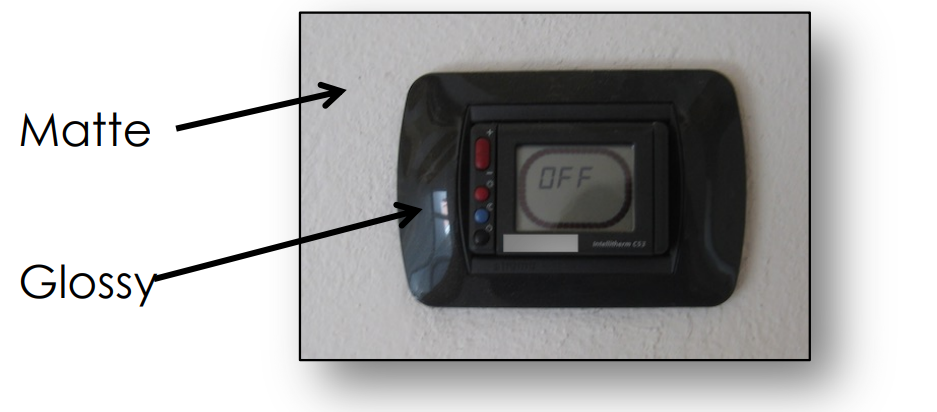
\includegraphics[width=0.4\textwidth]{Figures/matte.png}
    \caption{Reflections.} 
    \label{fig:matte}
\end{figure}

Modeling surface irradiation by the light source involves determining how the light interacts with the surface. 
Assuming a distant light source, we can represent all rays with a single unit vector. 
Each surface element receives light based on the cosine of the angle between the surface normal and the light direction, affecting its perceived brightness and color.

\[
  i = n\cdot s  
\]
\begin{figure}[h]
    \centering
    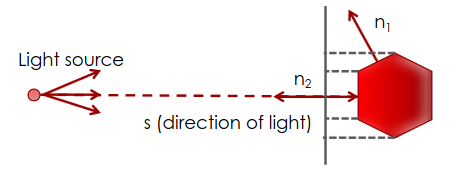
\includegraphics[width=0.5\textwidth]{Figures/Illumination.png}
\end{figure}
\\\textit{NB: intensity we perceive is equal to dot product of the normal of the surface and the light direction. Dot product $\Rightarrow$ cosine $\Rightarrow$ the more close to 90 degrees, the less we see.}
\subsection{Lambertian Reflectance}
Lambertian Reflectance is a model used to describe diffuse reflection. It operates under the assumption that the surface is sufficiently rough compared to the wavelength of light. In this scenario, each surface element reflects light uniformly in all directions, regardless of the viewing angle. This means that the luminance of the surface remains constant, irrespective of how it is observed. 
This model neglects any specular component of reflection, focusing solely on the diffuse characteristics of the surface.
\\\textit{NB: Assumes that the surface we're dealing with is ideal, so looking at it from any angle we'll see the same intensity.}
\[
    I = \rho n \cdot s = |n||s|\cos(\alpha) 
\]
Where:
\begin{itemize}
    \item $I$ is the intensity of the light;
    \item $\rho$ is the albedo, the ratio of the reflected illumination to the total illumination, intrinsic property of the surface (\textit{LOL not true, some surfaces may reflect light differently depending on the view angle});
    \item $n$ is the normal to the surface;
    \item $s$ is the direction of the light.
\end{itemize}

An element is not visible if the angle between the normal and the light direction is greater than 90 degrees.
Generally, the pixel in image $I(r,c)$ depends on the light source direction and the normal of the element direction.

\section{Remarks on cameras and lenses}
Cameras use lenses rather than pinholes, that do not exist in real life. This introduces the concept of \textbf{focus}. 
According to the thin lens equation, an object is in focus if the distance from the center of the camera to the image plane satisfies certain conditions. 
If this is not the case, it leads to \textbf{aberrations}, which are deviations from the ideal imaging process.
\\
While we usually assume that the object is in focus, it's important to understand the implications of this assumption. 
By adhering to the principles of the thin lens equation, we ensure that the camera captures images with minimal aberrations, resulting in clear and accurate representations of the scene.
\subsection{Typical issues with lenses}

\begin{wrapfigure}{r}{0.5\textwidth}
    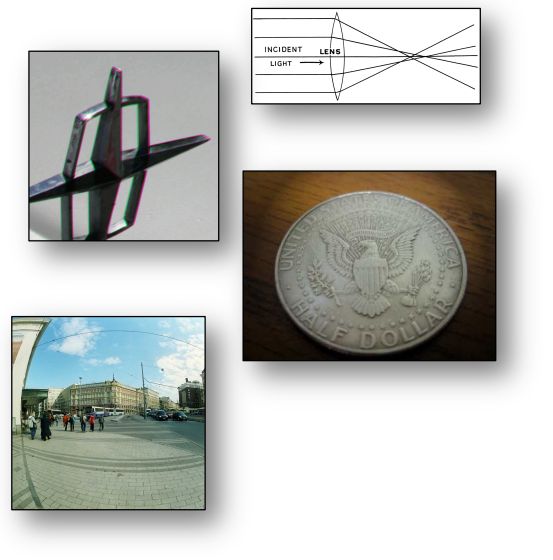
\includegraphics[scale=0.4]{Figures/ops.png}
\end{wrapfigure}

\textbf{Spherical aberration:} 
\\The lens does not focus light rays that strike the lens far from the center. This means that the image is not sharp (causes blur).
In simple terms the lens does not focus all the rays in the same point, so the light is reflected wrongly because the lens is not properly manufactured.
\\\textbf{Chromatic aberration:}
\\The lens does not focus all the colors in the same point, it's not able anymore to convey correctly the ray at different locations (for example cathode ray tube televisions).
\\\textbf{Vignetting:}
\\The lens does not focus all the rays in the same point, so the image is darker in the corners. The spreading of light is not uniform due to the impurity of glass.
\\\textbf{Barrel distortion:}
\\The focal length is too short or the lens is too wide, so the image is distorted and the lines are not straight anymore.
In simple terms, the lens is able to grasp a wide area of view. To compensate we can use a software to correct the distortion. 
\textit{NB: Crooked lines can give problems in path analysis\dots distortion problem $\Rightarrow$ that's why modern cellphones have more lenses.}
\subsection{Focus}
In contrast to the abstract pinhole model, real-life cameras employ lenses. These lenses have the remarkable ability to converge light rays to a single point, allowing for focused images. 
The relationship between the distance from the center of the camera to the image plane adheres to the thin lens equation.
\[
    \frac{1}{f} = \frac{1}{u} + \frac{1}{v}
\]
\begin{wrapfigure}[6]{r}{0.5\textwidth}
    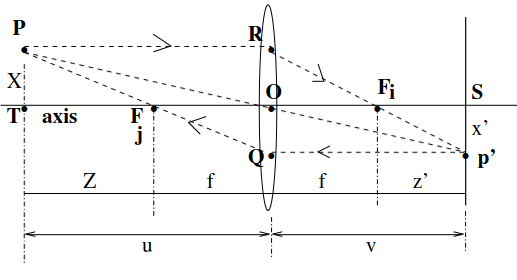
\includegraphics[scale=0.4]{Figures/ThinLenses.png}
\end{wrapfigure}

This equation serves as a fundamental principle in optics, ensuring that the lens accurately focuses incoming light onto the image sensor or film. 
It's this precise focusing mechanism that enables cameras to capture sharp and detailed images of the world around us.\\

If we move the image plane, point $p'$ is out of focus $\Rightarrow$ $v$ changes $\Rightarrow$ $v'$. And, if $P$ is moved $u$ changes $\Rightarrow$ $u'$.
The result is that the image is blurred on the image plane (instead of a point I see a circle, the rays of light don't converge).
\\\textit{NB: If the object is too far you can try to set the focal length but it won't work.}
\begin{figure}[h]
    \centering
    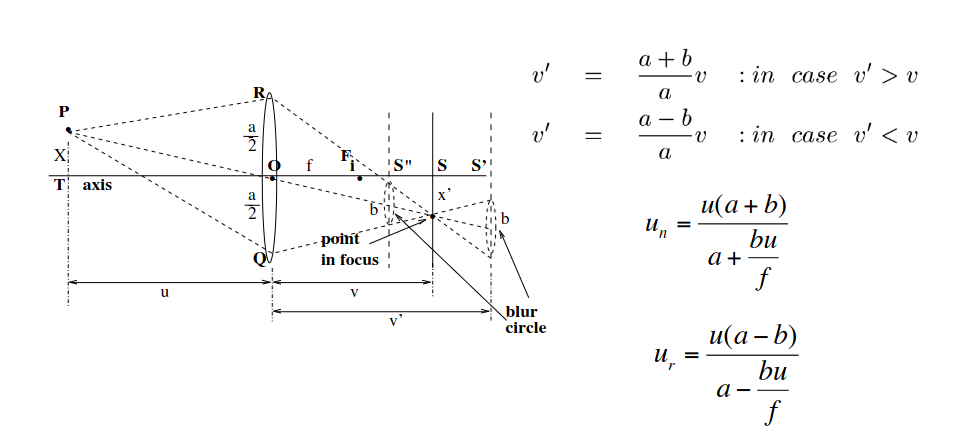
\includegraphics[width=1\textwidth]{Figures/Focus.png}
\end{figure}
\\We want to configure the camera in order to have the quantity $b$ as small as possible.
\\Notice that:
\begin{itemize}
    \item In general $u > f = u_n < u$;
    \item If $f$ becomes smaller, $u_n$ is closer to the camera;
    \item If $f$ becomes smaller, $u_r$ is farther to the camera;
    \item $u_r > u$;
    \item If $u -> \infty$ rays are parallel and converge to the camera center;
    \item The difference between the far and near planes limiting b is called \textbf{depth of field}. 
\end{itemize}

\textbf{Autofocus}
\\Is the capability of focusing a specific portion of the image, it can be active, passive or a combination of both.
\begin{quote}
    \textbf{Active:}  
    \\The camera emits a signal and measures the time it takes for the signal to return, using this time to calculate the distance to the object. 
    This method is commonly used in point-and-shoot cameras. 
    However, it faces challenges with obstacles, glossy surfaces, and bright reflections, which can interfere with accurate distance measurement.
\end{quote}
\begin{quote}
    \textbf{Passive:}
    \\Professional cameras use image contrast to achieve focus, primarily employing the phase detection method. 
    This technique, commonly found in expensive SLR (single-lens reflex) cameras, involves analyzing a strip of pixels to assess contrast levels. 
    If pixel values are too similar, the object is out of focus; if the contrast is high, the object is in focus.
    \\
    This method faces challenges with flat surfaces, low contrast, and low light conditions. 
    High-quality cameras address this by computing focus metrics along both vertical and horizontal axes to ensure accurate focusing.
\end{quote}

\subsection{Resolution, Blur and Resolving Power}

We might have blurring due to the focus problem described in the previous section, but also due to the quality of the sensor. A CCD sensor of size $N\times M$ can detect up to $N/2$ horizontal lines, meaning that in order to differentiate two lines there must be some spacing between them, one pixel at minimum, so given $N$ rows of pixels only half of them can be filled with lines.

\begin{figure}[H]
    \centering
    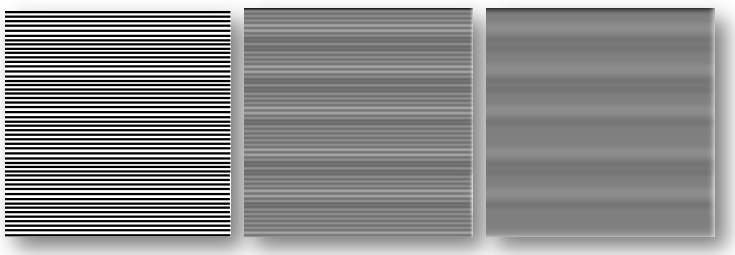
\includegraphics[width=0.7\textwidth]{Figures/blur.png}
    \caption{The right images are blurred because the sensor is not able to distinguish the lines.}
    \label{fig:blur}
\end{figure}

The \textbf{resolving power} of a camera is the ability to distinguish between two points, it is defined as:


\begin{multicols}{2}
\[
    R_p = \frac{1}{2\Delta}\;\;\; [lines/mm]     
\]
\begin{figure}[H]
    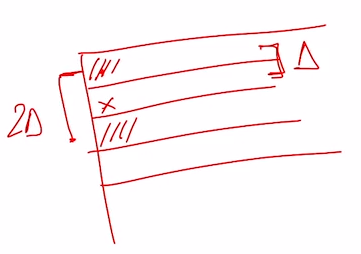
\includegraphics[scale=0.3]{Figures/separation.png}
\end{figure}
\end{multicols}

Where $\Delta$ is the pixel spacing: the distance between two pixels/lines in the sensor. The reason why we divide by 2 is that we need one separating row of pixels between two lines.

\textbf{Example}
\\
% \begin{wrapfigure}[115]{r}{0.3\textwidth}
%     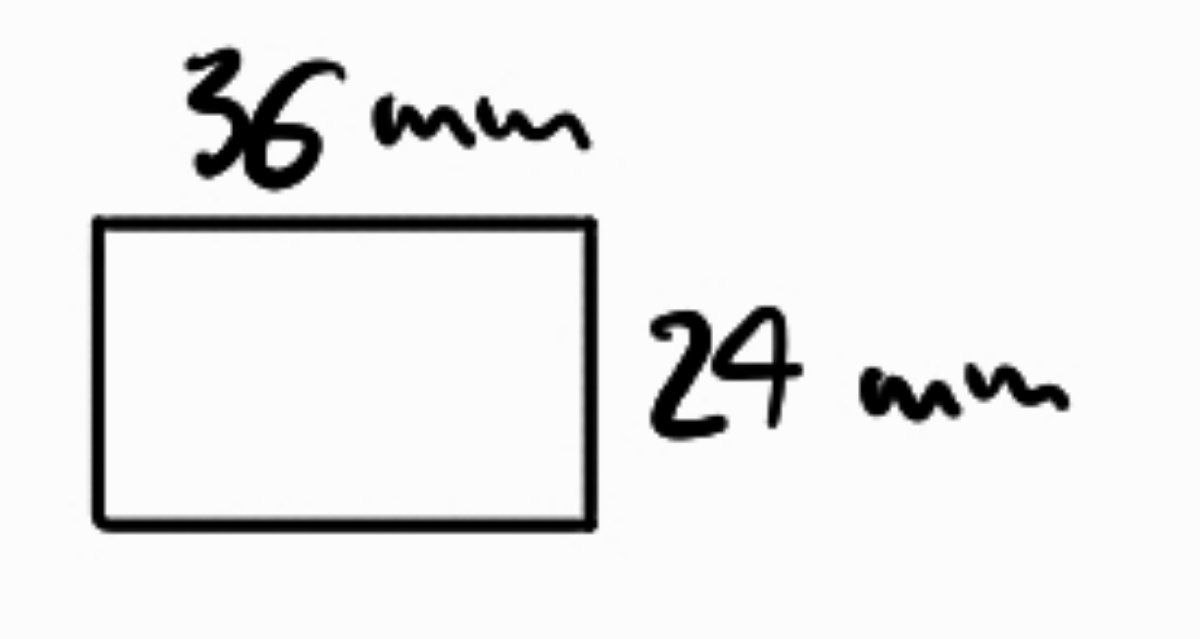
\includegraphics[scale=0.1]{Figures/sensor.png}
% \end{wrapfigure}
Camera \(10Mpx \; \rightarrow \; 4000 cols \times 2500 rows \) \\
Full frame sensor \(\rightarrow \; 36mm \times 24mm \)

\[
    R_p = \frac{1}{2\Delta} \;\;\; \Delta = \frac{24}{2500} \approx 0.01mm 
\]
\[
    R_p = \frac{1}{2 * 0.01} = 50 \; \frac{lines}{mm}    
\]

This means our sensor can distinguish 50 lines per millimeter, now we want to place our sensor in a camera in the real world and understand how well we can perceive details. Our setup is the following:\\
Focal length \(f = 50mm\) \\
Distance from the object \(L = 50m = 5000mm\) \\

\begin{figure}[H]
    \centering
    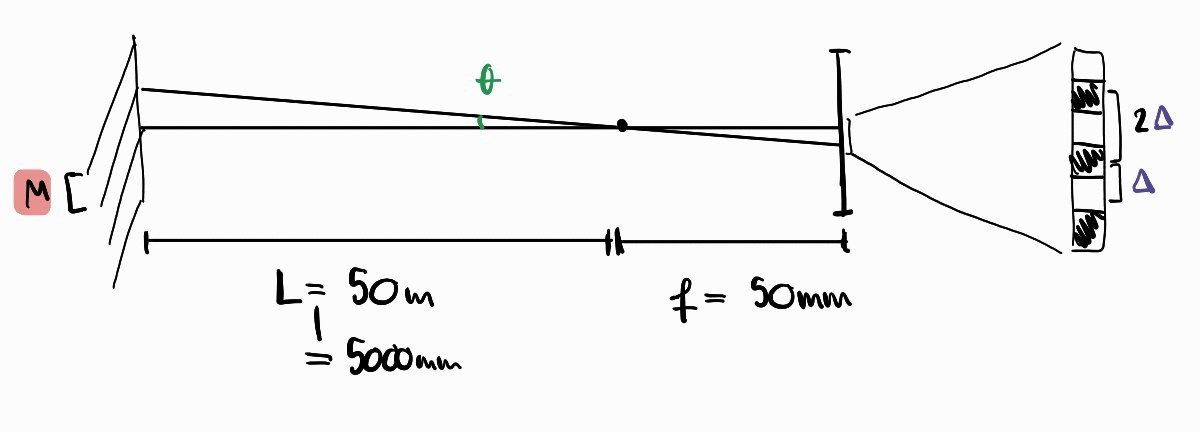
\includegraphics[width=0.8\textwidth]{Figures/rp.png}
    \caption{On the left we have a wall with some stripes, on the right we have our camera and sensor.}
    \label{fig:rp}
\end{figure}

We can see we have an angle \(\theta\) separating the rays coming from two adjacent lines. In order to distinguish two lines, the spacing between pixel lines must be at least \(2\Delta\), we can write:

\[
    2\Delta = f \sin(\theta)
\]

Since the angle is very small, the sine can be approximated to the angle itself. We can now calculate:

\[
    2\Delta \approx f\theta = 50\theta
\]

We can now determine the angle \(\theta\):

\[
    \theta = \frac{\Delta}{25} \approx 4 * 10^{-4} rad
\]
Now that we have the angle and we know the distance from the object to the camera, we can calculate what is $M$, the distance between two lines on the wall:

\[
    M \approx L\theta = 5000 * 4 * 10^{-4} = 2mm    
\]

With this expression we are saying that, given this setup, I can distinguish two lines which are spread vertically by a quantity no smaller than $2mm$.